\documentclass[9pt,twocolumn,twoside]{osajnl}

\journal{jocn} 

% See template introduction for guidance on setting shortarticle option
\setboolean{shortarticle}{false}
% true = letter / tutorial
% false = research / review article
% (depending on journal).

\title{ \emph{Advancement of Smartphone Security Using Iris Scan Detection  }}

\author{Mohit Mehta}

\affil{Publications Department, Christ University, 1969  S.G. Palya, Bengaluru, Karnataka 560029, India}
\affil{Department of Computer Science,Christ University, 2022  S.G. Palya, Bengaluru, Karnataka 560029, India}

\affil[*]{Corresponding author: mohit.mehta@mca.christuniversity.in}

%% To be edited by editor
\dates{Compiled \today}

%\ociscodes{(140.3490) Lasers, distributed feedback; (060.2420) Fibers, polarization-maintaining;(060.3735) Fiber Bragg gratings.}

%% To be edited by editor
% \doi{\url{http://dx.doi.org/10.1364/XX.XX.XXXXXX}}

\begin{abstract}
Mankind does have a habit of inventing new eras to get to being simpler and more satisfying. As a means of protecting this generation, security gadgets play a key role. In this technology, the device combines biometrics as well as a virtual code lock that responds in real time to code matching or mismatching. The goal of these research is to explore into human-computer interaction. Eye tracking is becoming quite significant method of analysing human behaviour. A proper study of statistics acquired from a watch tracker, on the further note, a complex undertaking. . In this chapter, we'll cover some of the ways, that how Iris scanners are being utilised for biometrical analysis and are being monitored with the help of a microcontroller and biometric sensors.
\end{abstract}

\setboolean{displaycopyright}{true}

\begin{document}

\maketitle

\section{Introduction}
As far as we speak of humans all we have three such things which differ in all of us, the first is 'DNA' second is our 'fingerprint' and the third is the 'pattern of our iris'. In a typical 'Fingerprint scanner' application for biometric access, we must grant or deny access to a specific person. We don't use the 'DNA' we use in forensic research in everyday life because it's too difficult to use. 'IRIS SCANNING' is the last choice we have. If we're talking about regular consumer products and day-to-day living, we can conduct fingerprint scanning, iris scanning, or both. 

When we speak about IRIS scanner it is not so common that it will see us in a little specific place. This technology, however, is more secure than a fingerprint scanner. When compared to
fingerprint scanning, it is far faster and more efficient. Now let's look at how an iris scanner works. Look at the pattern in the middle of our eyes, blue eyes, black eyes, or what we call an iris. The fine granular components that make up this pattern differ from person to person. This iris does not change till a person dies; it remains the same throughout their lives. 

The principle is the same as fingerprint scanning in that we scan the iris once, compare it to the result of the next scan, and the system tells us if the results are a match or not. To scan a single fingerprint, however, at least 40 to 45 points must be scanned. The iris scanner system scans at least 200 to 250 points to identify the user. It is compatible with high-level security until all the conditions are met.

Now understand how a scanner works: it has an infrared camera and a regular camera, both of which take an extremely high-resolution photo of your iris and pick up essential data such as diversions, arcs, and curves, which it detects. Make a code called the iris code after scanning these 240 to 250 spots. For example, if individual 'A' scans his or her iris, the system generates a code for that person. It will be named code for the individual 'A' after encryption. When person 'A' goes for iris scanning on the same system or mobile the next time, both cameras take pictures of the iris again, this information is converted into a code again, and the system checks all scanned codes and compares them to other saved scanned until they match the code of person 'A' or not. The system displays an error notice if the code does not match the saved scanned code.

\section{Literature Review}
The goal of the literature review is to identify problems with feature extraction and learn about current challenges in iris recognition. To be aware of what new iris recognition technologies can be applied to mobile devices.

Neda Ah. \cite{Chitimalla:17} Proposed a brand-new technique for classifying iris pictures based on MLPNN and PSO. The feature extraction process made use of the 2D kernel algorithm. The hybrid MLPNN-PSO algorithm is an efficient, appropriate, stable, robust, and competitive recognition approach for human iris recognition, according to testing on the iris V3 database and machine learning repository datasets. In comparison to using the MLPNN and PSO algorithms separately, the hybrid approach produced better experimental results. A suitable classifier must be discovered for the proposed technique in order to improve the proposed algorithm's effectiveness and success.

\begin{figure}[htbp]
\centering
\fbox{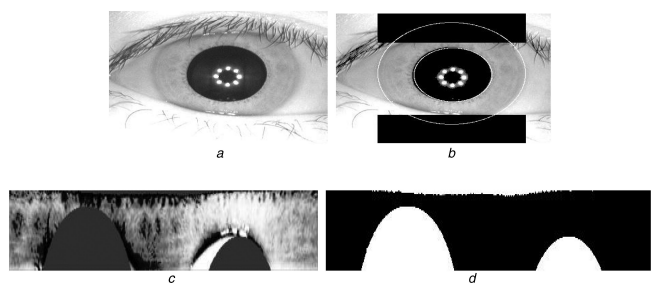
\includegraphics[width=.8\linewidth]{1.png}}
\caption{Iris normalisation (a) Original image, (b) Noise removal, (c) Polar coordinate, (d) Polar coordinate noise}
\label{fig:Iris normalisation}
\end{figure}

Upal Ma. \cite{Wen:16} Surveyed into the effects of unidentified applications and unexpected observations on the authentication problem has revealed that the addition of uncertain occurrences is important for this challenge to get better results. The trials produced some quite intriguing findings regarding the variations between the two datasets. The research also discussed various facets of crucial real-world factors as intrusion detection, latency, observation history, and sampling rate.

\begin{table}[htbp]
\centering
\caption{\bf Comparison of different biometric technology.}
\begin{tabular}{ccc}
\hline
Biometrics & Crossover Accuracy  \\
\hline
Retinal Scan & 1:10,000,000+ \\
Iris Scan & 1:131,000 \\
Fingerprints & 1:500 \\
Hand Geometry & 1:500 \\
Signature Dynamics & 1:50 \\
Voice Dynamics & 1:5 \\
\hline
\end{tabular}
  \label{tab:shapefunctions}
\end{table}

Jasem Ra. Ma. \cite{sam:3} To reiterate, the IRIS has seven main phases: the acquisition phase of the iris image, the preprocessing phase to enhance the image, the iris segmentation phase to separate the iris region from the eye image, the normalization phase to turn the segmented iris region into a rectangular pattern, the feature extraction phase to extract the iris features, the feature selection phase to select the unique features, and the classification/matching phase to find the similarity between the iris image and images in databases.

\begin{figure}[htbp]
\centering
\fbox{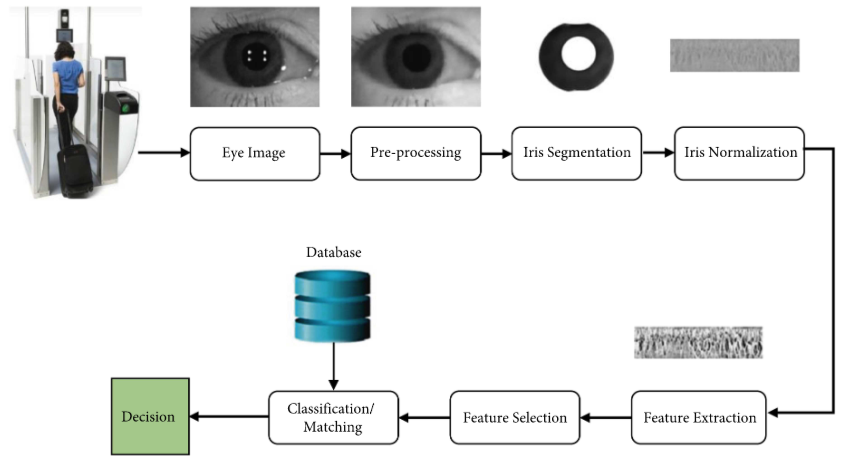
\includegraphics[width=.8\linewidth]{2.png}}
\caption{A fundamental structure of the iris recognition system (IRS).}
\label{fig:Fundamental Structure}
\end{figure}

Ehsaneddin Ja. \cite{sam:4} The results produced using the modified homogenous technique demonstrated that the network's performance is directly correlated with how closely the gaze angles of the training and testing images match and degrades as they diverge. We also discovered that as the gaze angle of the training and testing data converges in terms of angle but diverges in terms of direction, the network performance gradually improves. As a result of the segmentation enhancement, it was determined that the network was able to recognise the symmetric iris contents in photos taken from the same angle but in the opposite direction. These are, in fact, very promising results, as the selected approach enabled us to refrain from (i) the angle‐specific training strategy, which requires determination of the iris images gaze angles in advance, and (ii) even more important, carrying out the correction procedure.

\begin{figure}[htbp]
\centering
\fbox{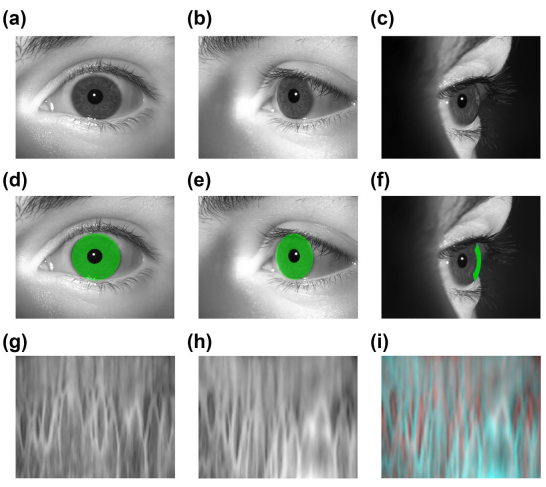
\includegraphics[width=.8\linewidth]{3.png}}
\caption{Examples of the iris images in the dataset and the corresponding off‐angle distortions.}
\label{fig:Examples of Distortions}
\end{figure}

Reend Ta. \cite{sam:5} Surveyed the irises that are matching if the Hamming distance between the two templates is 0.0; else, the two templates do not match. We can infer from the research given in this paper that the placement and lighting variations for particular datasets cause some errors in the recognition system. The best results were obtained using the MMU and CASIA, MICHE I DATASETS, which were especially taken for the recognition system. In contrast, the lower-quality iPhone camera photographs were not as successful due to poor location and illumination. The late recognition in comparison to the MMU and CASIA dataset was the sole negative.

\begin{figure}[htbp]
\centering
\fbox{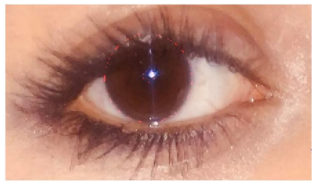
\includegraphics[width=.8\linewidth]{4.png}}
\caption{Iris images from external data have been taken by iPhone camera. Localization is done for the left eye by using Daugman's operator which takes 47.0799 s}
\label{fig:I-Phone}
\end{figure}

\begin{figure}[htbp]
\centering
\fbox{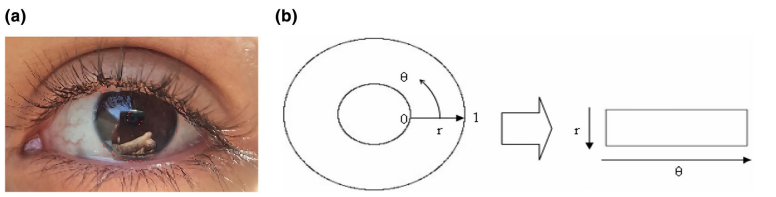
\includegraphics[width=.8\linewidth]{5.png}}
\caption{(a) Iris image from external data have been taken by an Android camera. Localization is done for the left eye by using Daugman's operator which takes 143.0010 s. (b) Daugman's Rubber Sheet Model}
\label{fig:Android}
\end{figure}

Christian Ra. \cite{sam:6} The application of the general adaptive Bloom filter-based transform to the binary feature vectors of various iris recognition algorithms allows for I template protection, (ii) biometric data reduction, and (iii) computationally efficient biometric identification. The methods currently used to preserve iris biometric templates are either unsecure or have poor biometric performance. On the other hand, the suggested rotation-invariant Bloom filter-based transform offers a high level of security while maintaining recognition accuracy. Additionally, the proposed technique may be parameterized to greatly reduce the size of biometric templates. Additionally, since bit-shifting is no longer used at the moment of the biometric comparison, the process of biometric identification is significantly sped up.

\begin{figure}[htbp]
\centering
\fbox{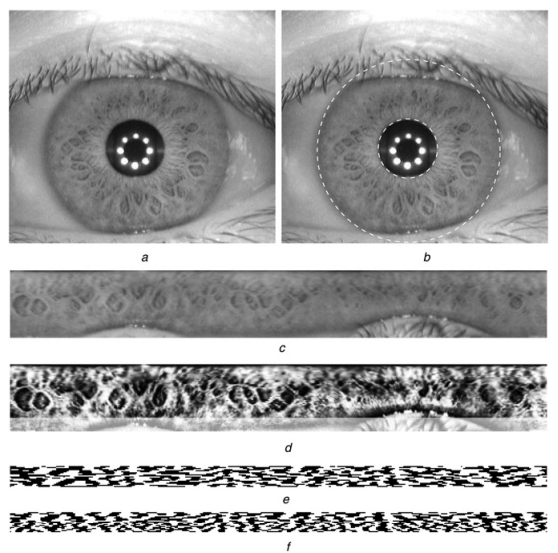
\includegraphics[width=.8\linewidth]{6.png}}
\caption{Preprocessing and both applied feature extraction algorithms
(a) Acquisition
(b) Detection
(c) Iris texture
(d) Pre-processed iris texture
(e) Iris-code 1D Log-Gabor Filter
(f) Iris-code Ma et al.}
\label{fig:Gabor}
\end{figure}

 Weizhi et.al. \cite{sam:1} Surveyed the development of existing biometric authentication techniques on mobile phones, particularly on touchenabled devices, with reference to 11 biometric approaches (five physiological and six behavioural). They presented taxonomy of existing efforts regarding biometric authentication on mobile phones and analyze their feasibility of deployment on touch-enabled mobile phones. In addition, they systematically characterized a generic biometric authentication system with eight potential attack points and survey practical attacks and potential countermeasures on mobile phones.

\section{ Conventional iris Matching systems}

The similarity of two given IrisCodes is assessed in the matching step. A similarity score is generated by computing the Hamming distance between two IrisCodes IC A and IC B as follows: 

\begin{equation}
HD = \frac{||(IC_A + IC_B) + M_A + M_B||}{||M_A + M_B||}
\label{eq:refname1}
\end{equation}

The terms denote the corresponding normalized noise masks. If two bit patterns are completely independent (i.e., IrisCodes generated from different irides), the Hamming distance should be equal to 0.5. If the IrisCodes are from the same iris, the Hamming distance should be 0

\section{Conclusion}

The main intension of this paper research is the development of reliable recognition based on iris images captured, without requiring the subject’s cooperation and under heterogeneous lighting conditions in an uncontrolled environment.The dynamics of the imaging environments cause very diverse images to arise, with the iris information being distorted by a variety of noise sources, including dilated pupils, eyelashes, eyelids, and image rotation from head tilt and camera rotation. Numerous publications have noted that the challenge of executing reliable recognition is greatly increased by these images.

% Bibliography
\bibliography{sample}
  
\end{document}
